\documentclass[11pt]{article}

\usepackage[margin=1.1in]{geometry}
\usepackage{amsmath}
\usepackage{booktabs}
\usepackage{graphicx}
\usepackage{microtype}
\usepackage[round]{natbib}
\usepackage[hidelinks]{hyperref}
\usepackage{caption}
\captionsetup{font=small, labelfont=bf, width=.92\textwidth}
\usepackage{orcidlink}

\newcommand{\code}[1]{\texttt{#1}}

\title{Forecasting the Supreme Court with Honest Features:\\
Walk-Forward Vote Prediction, Coalition-Aware Aggregation,\\
and a Live Two-Stage Preregistered Registry}

\author{Kara Zajac\,\orcidlink{0009-0001-7400-1394}\\
\small Independent researcher \quad \href{mailto:kara@soulstone.org}{kara@soulstone.org}}

\date{Draft of July 2026\thanks{Code, data, and every validation artifact:
\url{https://github.com/KaraZajac/JUDGMENT}; archived at
\href{https://doi.org/10.5281/zenodo.21211376}{doi:10.5281/zenodo.21211376}.
Live forecasts: \url{https://judgment.karazajac.io}.}}

\begin{document}
\maketitle

\begin{abstract}
\noindent We present JUDGMENT, an end-to-end system for forecasting Supreme Court
behavior at the level of individual justice votes and case outcomes, built on the
Supreme Court Database (SCDB) and evaluated exclusively by walk-forward validation
over 69 terms (1956--2024). A gradient-boosted model restricted to strictly
pre-decision features attains \textbf{67.9\% justice-vote accuracy} (Brier 0.207)
and \textbf{69.4\% case-outcome accuracy} in its deployed cert-stage configuration
--- exceeding our own full-SCDB research configuration and decisively beating
base-rate, justice-history, and attitudinal baselines (case-clustered bootstrap,
$+3.3$ points over the strongest baseline, 95\% CI $[+2.7, +3.8]$). A separately
validated \textbf{post-argument stage} adds per-justice questioning features parsed
from 7{,}023 oral-argument transcripts and the side the Solicitor General supports
as amicus, reaching \textbf{69.6\% justice-vote accuracy} (Brier 0.200,
AUC 0.723); the SG signal alone is worth $+5.2$ points where it applies, and the
combination resolves a format regime change that had erased questioning signal
in the post-2020 seriatim era. Four methodological contributions travel beyond
this system. First, \emph{deployment honesty}: the configuration that publishes
forecasts is restricted to features actually knowable for a pending case and is
validated separately; the unrestricted model produces degenerate forecasts under
deployment missingness. Second, a \emph{two-factor coalition model} over calibrated
per-justice marginals replaces the ubiquitous vote-independence assumption,
improving out-of-sample split-distribution log-loss by 45\% while also improving
binary outcome accuracy. Third, an \emph{audited adoption gate}: every candidate
feature faces the same walk-forward test, five rejections are documented alongside
four adoptions, and a nested-selection replay shows the entire adoption sequence
reproduces itself when decided on pre-2011 evidence alone --- scoring 71.5\%
justice-vote accuracy on the untouched 2011--2024 window. Fourth, a \emph{live
two-stage preregistered registry}: cert-stage forecasts freeze on argument day,
post-argument forecasts re-register separately, and a strictly ex-ante scoring
rule --- enforced in code, exercised by its first real case --- makes post-hoc
revision both detectable and inert.
\end{abstract}

\vspace{.5em}
\noindent\textbf{Keywords:} Supreme Court, judicial behavior, forecasting,
walk-forward validation, calibration, oral argument, preregistration.

\section{Introduction}

Quantitative prediction of Supreme Court behavior has a distinguished lineage:
ideal-point models of judicial ideology \citep{martinquinn2002}, pre-confirmation
ideology scores \citep{segalcover1989}, the statistical-models-versus-experts
contest of the 2002 term \citep{ruger2004}, and general machine-learning models
spanning two centuries of decisions \citep{katz2017}. Yet published systems are
difficult to audit \emph{as forecasters}: evaluations vary in leakage discipline,
probability calibration is rarely reported, case-level probabilities are almost
universally computed under an indefensible independence assumption across the
nine votes, and --- most fundamentally --- retrospective accuracy does not
establish that a system's \emph{deployable} configuration, facing the information
actually available before decision, performs as advertised.

This paper describes a system built to be auditable in exactly those respects,
and reports what such discipline reveals. Our contributions:

\begin{enumerate}
\item \textbf{A leak-free evaluation harness} (\S\ref{sec:methods}): walk-forward
  only --- train on terms $\le T{-}1$, predict every vote of term $T$ --- with an
  explicit feature-availability policy and prospective recalibration.
\item \textbf{Deployment honesty} (\S\ref{sec:deployment}): the published
  forecaster is a separately validated configuration restricted to
  stage-appropriate features. We document that the full research model, whose
  accuracy headlines would normally be quoted, collapses to degenerate output
  under deployment missingness --- a failure mode invisible to standard
  evaluation.
\item \textbf{Coalition-aware aggregation} (\S\ref{sec:coalition}): a two-factor
  probit structure over calibrated marginals that recovers the Court's unanimity
  modes without sacrificing --- indeed while improving --- binary outcome accuracy.
\item \textbf{An audited feature-adoption gate} (\S\ref{sec:gate}): four
  adoptions and five documented rejections under one protocol, including a
  twice-tested negative result for question text, the measurement of the
  Solicitor-General-as-amicus effect, and the discovery and resolution of a
  format regime change in oral argument.
\item \textbf{A methods audit} (\S\ref{sec:audit}): the three sharpest
  criticisms we could level at our own procedure --- adaptive selection on a
  reused validation window, clustered dependence in significance tests, and an
  unvalidated attribution heuristic --- each converted into an experiment and
  answered.
\item \textbf{A live two-stage preregistered registry} (\S\ref{sec:registry}):
  forecasts for every granted-but-undecided case, timestamped in a public git
  history, with cert-stage forecasts frozen at argument, post-argument forecasts
  scored as their own track, and a strictly ex-ante scoring rule enforced in code.
\end{enumerate}

\section{Related work}\label{sec:related}

\paragraph{Ideal points.} \citet{martinquinn2002} introduced dynamic Bayesian
item-response modeling of justices' latent positions; their scores are the
field's standard ideology measure. We re-estimate ideal points in a penalized-ML
variant of their model rather than consuming published scores, attach
parametric-bootstrap uncertainty, and test their \emph{predictive} contribution
--- which proves nil beyond lagged behavioral rates, an instructive redundancy.

\paragraph{Prediction.} \citet{ruger2004} showed simple classification trees
beating a panel of experts on the 2002 term (75\% vs.\ 59\% case accuracy).
\citet{katz2017} built time-evolving random forests over SCDB features for
1816--2015, reporting 70.2\% case and 71.9\% justice-vote accuracy out-of-sample;
theirs is the benchmark general model, but two regime differences make the
comparison indicative rather than head-to-head: their feature discipline is
decision-date knowability rather than cert-stage (features include whether oral
argument was heard, whether a rehearing occurred, and the elapsed time from
argument to decision), and their margin over the always-petitioner rule is
roughly two points \citep[whose survey characterizes it as ``a small improvement
over the 68\% baseline'']{medvedeva2023}. \citet{kaufman2019} report the highest
published academic figure --- 74.04\% case accuracy over 2005--2015 --- but the
entire above-baseline margin comes from oral-argument features: their
case-covariates-only model scores 60.6\%, \emph{below} the 67.98\%
always-petitioner baseline, under pooled ten-fold cross-validation rather than
walk-forward evaluation. Read against our results (\S\ref{sec:gate}), that
finding independently corroborates this paper's central negative result --- at
the cert stage, structure is nearly all there is, and predictive content arrives
with argument.

\paragraph{Crowds and markets.} The FantasySCOTUS crowd is the one system that
genuinely outperforms our numbers, and it does so on later information: over
OT2011--2016 (425 cases, 7{,}284 participants) fair aggregation rules score
$\sim$74.1\% case / 73.5\% justice-vote, with predictions revisable until the eve
of decision and no probabilities, Brier, or calibration reported
\citep{katz2017crowd}; the widely quoted 80.8\% is the authors' own post-hoc
ceiling across 277{,}201 aggregation configurations. Prediction markets provide
no systematic docket coverage. No verified LLM-based system reports accuracy
above ours \citep[60\% case]{hamilton2023}; the JUSTICE text benchmark reports
$\le 68\%$ despite augmented case variants straddling a random train/test split
\citep{alali2021}; and \citet{medvedeva2023} document that much of the wider
``legal judgment prediction'' literature classifies post-decision documents
rather than forecasting from pre-decision information. As of mid-2026, no
algorithmic system publishes live, calibrated, preregistered forecasts of
pending cases; the registry of \S\ref{sec:registry} occupies an empty lane.

\paragraph{Oral argument.} That questioning at argument reveals the likely
outcome is well established: the side receiving more questions tends to lose
\citep{johnson2009, epsteinlandesposner2010}, and \citet{kaufman2019} built
their above-baseline margin on argument text. Our contribution is to measure
the signal per-justice, side-attributed, across seven decades under
walk-forward discipline --- and to document a format regime change that
compresses it (\S\ref{sec:oral}).

\section{Data}\label{sec:data}

\subsection{Canonical corpus}

The Supreme Court Database \citep{scdb2025} supplies 29{,}202 cases and 255{,}832
justice-vote records spanning the 1791--2024 terms. Our pipeline restructures the
corpus into per-case records (votes embedded, closed code sets decoded against
the SCDB codebook) and per-justice records combining curated biography with
computed voting histories. Structural validation --- identifier coherence,
vote-token validity, tally consistency against SCDB's own counts, membership
integrity --- runs on every build; residual soft findings are upstream SCDB
quirks and are documented rather than silently repaired. Justice biographies for
the modern era are hand-curated from public record; earlier justices are
enriched from the Federal Judicial Center's Biographical Directory.

\subsection{The living edge}

SCDB is released annually, so the term in progress is invisible to the canonical
dataset for months. Three ingestion layers close the gap, each writing records
flagged provisional and replaced wholesale when SCDB coverage arrives: Oyez
\citep{oyez} supplies decided-case metadata and (with days-to-weeks lag)
per-justice votes; CourtListener \citep{courtlistener} supplies near-real-time
decision events; and the Court's own slip-opinion syllabi are parsed for
same-day per-justice lineups. The syllabus parser is \emph{validation-gated}: it
must reproduce the lineups of independently coded cases before it may write
anything (it currently agrees on 43 of 44 such cases, 98\%). One subtlety
matters for correctness: every upstream source keys consolidated decisions to
the lead docket alone, so a map parsed from the syllabus's ``Together with
No.~\ldots'' footnote resolves companion dockets to their deciding record ---
seven such pairs in OT2025 alone.

\subsection{Auxiliary corpora}\label{sec:oralcorpus}

Question-presented texts for 3{,}418 historical cases support the text
experiments of \S\ref{sec:gate}. An \textbf{oral-argument questioning corpus}
covers 7{,}023 argued cases --- 96\% of the 1955--2024 terms, never below 94\%
in any decade --- parsed from Oyez's structured per-speaker transcripts into
per-justice, side-attributed turn and word counts. Sides resolve from advocate
descriptions where present; in the pre-1970s metadata gap they resolve from
argument order (petitioner opens and rebuts), a heuristic validated blind at
99.0\% section agreement on the two-advocate structure that dominates the era
it serves (\S\ref{sec:audit}). The same advocate metadata yields the side the
United States supports as amicus at argument (723 cases). Lower-court opinions
matched via docket-number joins accumulate as training data for a direction
classifier (in progress; the deployed system uses hand-coded direction with
documented bases).

\section{Methods}\label{sec:methods}

\subsection{Targets}

Primary: does justice $j$ vote to \textbf{disturb the judgment below} (reverse
family = reversed / vacated / partial reversals; affirm = affirmed), defined
where SCDB codes both disposition and majority membership --- the observable,
ideology-coding-free target comparable to \citet{katz2017}. Secondary: the SCDB
liberal/conservative \textbf{direction} of the vote, which inherits the Spaeth
coding conventions and their critiques. Case outcome is the majority side of
the (up to) nine votes.

\subsection{Features and the availability policy}

Every feature must be knowable \emph{before} the decision, and the deployed
configurations restrict further to features knowable at their stage:

\begin{itemize}
\item \textbf{Case features (cert stage)}: hand-codable issue area,
  jurisdiction, U.S.-as-party flags, and the ideological direction of the
  decision below --- the anchor for the latter being that certiorari petitioners
  lost below, classified under SCDB conventions, with ambiguous cases left
  honestly uncoded.
\item \textbf{Justice features}: computed from votes in terms strictly before
  the row's term (term-granular expanding windows): tenure, prior reverse rate,
  prior liberal share (career and last-3-terms, and within issue area), prior
  majority/dissent rates --- all empirical-Bayes shrunk toward running
  strictly-prior means --- plus the appointing president's party. First-term
  justices carry pure priors; the cold start is honest.
\item \textbf{Argument features (post-argument stage only)}: per-justice words
  and turns directed at each side while it held the floor; the justice's word
  share toward the petitioner minus her own lagged three-term mean share (so
  style and format norms cancel); bench-wide aggregates; and the side the
  Solicitor General supports as amicus.
\end{itemize}

Nothing downstream of the vote (disposition, direction, majority size, opinion
data) is ever a feature. We follow the literature --- and flag the optimism ---
in treating SCDB's post-hoc issue coding as cert-stage-knowable for historical
evaluation; the deployed forecaster uses hand-coded provisional issue areas
instead, and \S\ref{sec:audit} pre-commits to measuring the coding agreement
when SCDB's release covers the forecast terms.

\subsection{Walk-forward protocol}

No random splits, ever: random splits leak court composition and era effects.
For every evaluation term $T \in [1956, 2024]$ we train a gradient-boosted
classifier (histogram-based, native categorical and missing-value handling
\citep{pedregosa2011}) on all labeled votes from terms $\le T{-}1$ and predict
every vote of term $T$. Baselines are computed strictly from the same training
window: the training base rate; the justice's lagged shrunk prior rate; and the
classic attitudinal heuristic, $P(\text{reverse}) = P(\text{justice disagrees
with the ideological direction of the decision below})$. Features whose history
begins mid-window (e.g., the SG signal, sparse before the 1960s) simply sit out
training windows in which they are entirely missing.

\subsection{Prospective recalibration}

Raw model probabilities are recalibrated by isotonic regression fitted, for each
evaluation term $T$, only on out-of-sample predictions from terms before $T$ ---
exactly what a live forecaster could have done at the time. This reduces
vote-level expected calibration error to $\approx 0.02$--$0.03$ with slight
Brier improvements; Figure~\ref{fig:reliability} shows the resulting
reliability. The deployed calibrators are exported as portable step functions,
so any environment reproduces calibrated probabilities bit-exactly.

\subsection{Coalition-aware aggregation}\label{sec:coalition}

Aggregating nine per-justice probabilities under independence is indefensible:
it predicts 4.4\% unanimous reversals in a Court that is unanimous about a
third of the time. We place a two-factor probit coalition structure on top of
the calibrated marginals, preserving them exactly:
\begin{equation*}
\text{vote}_j \mid (u, v) \;\sim\;
\mathrm{Bernoulli}\!\big(\Phi(\mu_j + \lambda_0 u + \lambda_1 s_j v)\big),
\qquad
\mu_j = \sqrt{1 + \lambda_0^2 + \lambda_1^2 s_j^2}\;\Phi^{-1}(p_j),
\end{equation*}
where $u$ is a case-valence factor, $v$ an ideological factor, $s_j$ the
justice's lagged lean, and the loadings $(\lambda_0, \lambda_1)$ are fit on
walk-forward predictions from terms $\le 2010$ and evaluated strictly after.
Case distributions follow from two-dimensional Gauss--Hermite quadrature; no
Monte Carlo. Out-of-sample split-distribution log-loss improves by 45\%, and
--- non-obviously --- binary case accuracy improves as well (69.0\% $\to$
69.4\%): it is strictly better, not a sharpness trade
(Figure~\ref{fig:splits}).

\subsection{Deployment honesty}\label{sec:deployment}

The configuration that publishes forecasts is \textbf{pinned} --- never inferred
from artifact presence --- and is validated end-to-end like every other
configuration, with its own out-of-sample predictions supplying its calibrator.
This discipline is not decorative. When the full research model was first
pointed at pending cases, its never-seen missingness constellation (absent
lower-court codings, party codes, court codes) routed into unreliable leaves
and produced degenerate $\approx 1.00$ forecasts for every case --- a
catastrophic failure invisible to conventional evaluation, caught only because
deployment was treated as its own validated configuration. The deployed
cert-stage subset in fact \emph{outperforms} the full research configuration
(67.9\% vs.\ 66.8\% justice-vote), a lean-model result that recurs throughout
\S\ref{sec:gate}.

\section{Results}\label{sec:results}

\subsection{Headline performance}

Table~\ref{tab:headline} reports walk-forward vote-level performance over
1956--2024; Figure~\ref{fig:accuracy} shows the time path. The deployed
cert-stage configuration beats the strongest baseline by $+3.3$ points
(case-clustered 95\% CI $[+2.7, +3.8]$; \S\ref{sec:audit}), and the
post-argument configuration adds a further $+1.7$ points overall --- much more
where its information applies (\S\ref{sec:oral}).

\begin{table}[t]
\centering
\small
\begin{tabular}{lccccc}
\toprule
 & Accuracy & Brier & Log loss & AUC \\
\midrule
\multicolumn{5}{l}{\emph{Baselines (reverse target)}}\\
Training base rate        & .646 & .229 & --- & .487 \\
Justice history (lagged)  & .646 & .227 & --- & .548 \\
Attitudinal heuristic     & .623 & .228 & --- & .664 \\
\midrule
\multicolumn{5}{l}{\emph{Models (reverse target)}}\\
Bare cert subset               & .644 & .224 & .640 & .601 \\
$+$ lower-court direction      & .678 & .208 & .603 & .686 \\
$+$ recent topic lean (deployed cert stage) & .679 & .207 & .602 & .688 \\
Post-argument stage (deployed) & \textbf{.696} & \textbf{.200} & \textbf{.587} & \textbf{.723} \\
\midrule
\multicolumn{5}{l}{\emph{Direction target (liberal)}}\\
Deployed cert stage            & .661 & .211 & .610 & .727 \\
Post-argument stage            & .680 & .207 & .603 & .744 \\
\bottomrule
\end{tabular}
\caption{Walk-forward vote-level performance, evaluation terms 1956--2024
($n = 75{,}787$ reverse-labeled votes; 78{,}874 direction-labeled). Case-level
accuracy of the deployed cert configuration under coalition aggregation is
69.4\% ($n = 7{,}645$ cases). Every model row is trained, predicted, and
calibrated strictly out-of-time.}
\label{tab:headline}
\end{table}

\begin{figure}[t]
\centering
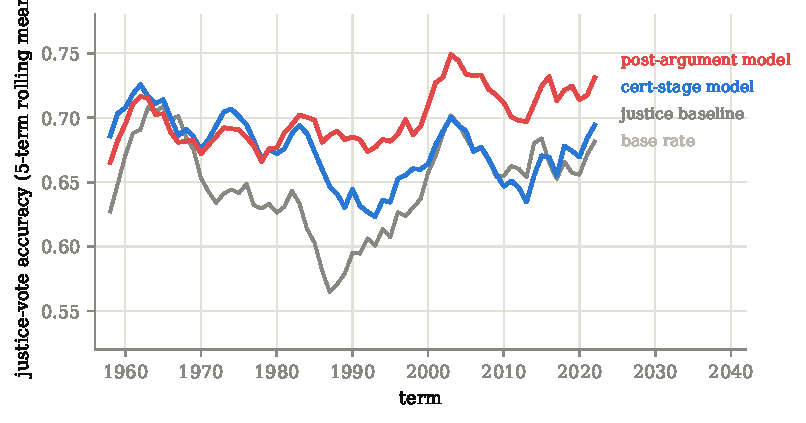
\includegraphics[width=.9\textwidth]{figures/accuracy-over-time.pdf}
\caption{Justice-vote accuracy by term (5-term rolling mean), walk-forward.
The cert-stage model's margin over the justice-history baseline is stable
across seven decades; the post-argument model's additional margin widens in
the modern era as transcript coverage and Solicitor General participation
grow.}
\label{fig:accuracy}
\end{figure}

\begin{figure}[t]
\centering
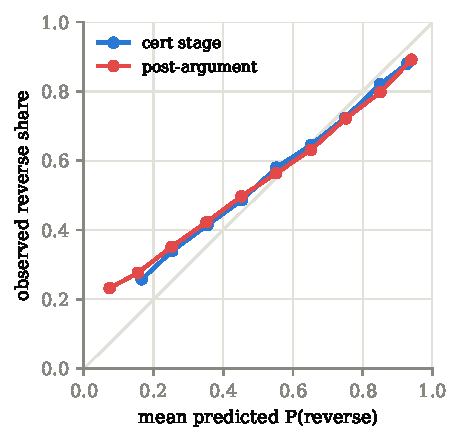
\includegraphics[width=.45\textwidth]{figures/reliability.pdf}
\caption{Reliability of the two deployed stages (decile bins, all evaluation
terms pooled). Prospective isotonic recalibration holds both stages close to
the diagonal.}
\label{fig:reliability}
\end{figure}

\begin{figure}[t]
\centering
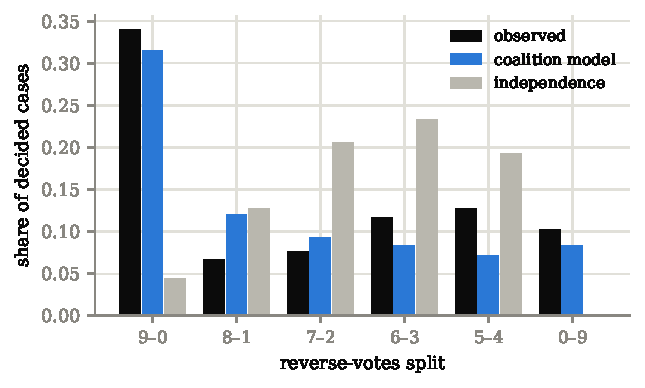
\includegraphics[width=.7\textwidth]{figures/splits.pdf}
\caption{Distribution of reverse-vote splits: observed, coalition model, and
independence aggregation of identical calibrated marginals. Independence
places 4.4\% on unanimous reversal against an observed 34.0\%; the two-factor
coalition model recovers both unanimity modes. Residual honesty: 5--4 mass
remains underpredicted.}
\label{fig:splits}
\end{figure}

\subsection{The feature-adoption gate}\label{sec:gate}

Every candidate feature faces the same protocol --- walk-forward evaluation on
both targets, judged on accuracy, Brier, and AUC --- and the ledger records
losers alongside winners (Table~\ref{tab:ledger}). Three findings deserve
narrative.

\begin{table}[t]
\centering
\small
\begin{tabular}{llll}
\toprule
Candidate & Stage & Verdict & Evidence (reverse target) \\
\midrule
Lower-court direction & cert & \textbf{adopted} & $+3.45$pp $[+3.02, +3.86]$ \\
Recent topic lean & cert & \textbf{adopted} & Brier/AUC; accuracy null \\
Question text (LSA), twice & cert & rejected & $-0.5$pp alone; no lc interaction \\
Segal--Cover nomination score & cert & rejected & null; first-term $+0.7$pp underpowered \\
Originating circuit & cert & rejected & worse on all six metrics \\
Lower-court dissent & cert & rejected & flat-to-worse both targets \\
Questioning (turns), oral & post-arg. & adopted$^{\dagger}$ & $+1.73$pp $[+1.11, +2.33]$ covered \\
Questioning (word-centric) & post-arg. & \textbf{adopted} & Brier everywhere; seriatim-robust \\
SG-as-amicus side & post-arg. & \textbf{adopted} & $+5.19$pp $[+3.32, +7.10]$ covered \\
Union (turns $+$ words $+$ SG) & post-arg. & rejected & worse direction-target profile \\
\bottomrule
\end{tabular}
\caption{The adoption ledger. Brackets are case-clustered bootstrap 95\%
confidence intervals (\S\ref{sec:audit}). $^{\dagger}$Turn-based questioning
was adopted and then superseded by the word-centric $+$ SG configuration.
Five rejections and four adoptions under one protocol; the file-drawer is
empty.}
\label{tab:ledger}
\end{table}

\paragraph{Structure beats content at the cert stage.} Question-presented text,
entered through leakage-safe per-step latent semantic features, does not improve
prediction either alone or --- refuting the interaction hypothesis directly ---
in the presence of lower-court direction. Meanwhile one hand-codable structural
judgment (the direction of the decision below) is worth $3.4$ points. Three
further cert-stage candidates --- a nomination-time ideology score, the
originating circuit, and the presence of a dissent below --- all failed the
same gate, the circuit categorical reproducing in miniature the variance
pathology that sank the full research configuration. Five straight rejections
of features that re-encode information already implicit in the lean
configuration constitute evidence of a \emph{cert-stage information ceiling}
near 68\% per-vote for this model class.

\paragraph{The questioning signal and a format regime change.}\label{sec:oral}
Per-justice questioning features add $+1.73$ points on transcript-covered votes,
with an era structure that is itself a finding
(Figure~\ref{fig:eras}): $+3.8$ to $+4.7$ points sustained across the
1980s--2010s --- the per-justice, walk-forward counterpart of
\citet{kaufman2019}'s case-level result --- negative in the 1950s--60s (cold
benches; heuristic attribution), and initially \emph{zero} in the 2020s. The
cause is mechanical: since OT2020 the Court appends seriatim justice-by-justice
questioning rounds to free-for-all argument, compressing turn-count
asymmetries. Word-volume features with a within-justice lagged baseline (so
format and style norms cancel), combined with the SG signal below, lift the
2020s covered slice from 68.6\% to 72.5\% (Brier $0.2045 \to 0.1872$): the
current Court's format becomes the model's best modern era rather than its
weakest.

\paragraph{The Solicitor General effect, measured.} The side the United States
supports as amicus at argument is the strongest single feature we have tested:
$+5.19$ points on covered votes (95\% CI $[+3.32, +7.10]$). The mechanism is
the classic one \citep{epsteinlandesposner2013}, here measured within our own
corpus: justices vote to reverse 75.8\% of the time when the SG backs the
petitioner and 42.3\% when it backs the respondent
(Figure~\ref{fig:sg}), and the model prices the swing almost perfectly (73.6\%
/ 44.7\% predicted). Because merits amicus participation is not knowable at
cert, the feature belongs to the post-argument stage --- whose transcript
harvest is also, conveniently, its data source.

\begin{figure}[t]
\centering
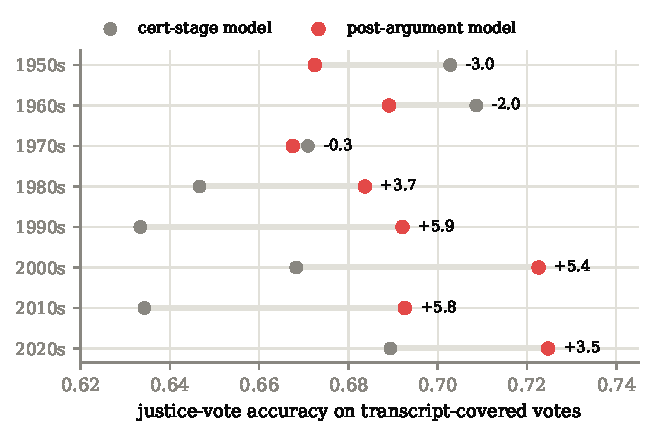
\includegraphics[width=.62\textwidth]{figures/era-dumbbells.pdf}
\caption{Justice-vote accuracy on transcript-covered votes by decade: deployed
cert-stage model vs.\ the deployed post-argument model. The post-2020
seriatim format initially erased the questioning signal; word-centric
features with a within-justice baseline plus the SG signal make the 2020s the
strongest modern era.}
\label{fig:eras}
\end{figure}

\begin{figure}[t]
\centering
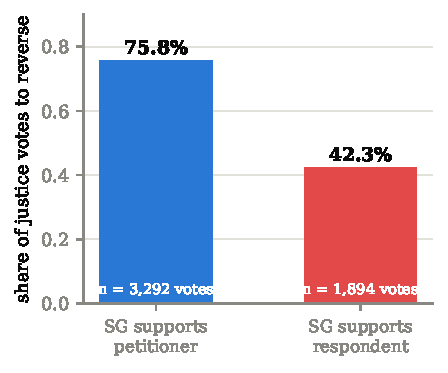
\includegraphics[width=.42\textwidth]{figures/sg-effect.pdf}
\caption{The Solicitor General effect in the corpus: share of justice votes to
reverse conditional on the side the United States supports as amicus at
argument (1955--2024; 723 cases).}
\label{fig:sg}
\end{figure}

\subsection{A methods audit}\label{sec:audit}

Three criticisms of our own procedure were converted into experiments.

\paragraph{Adaptive selection.} Every gate above reuses the same 1956--2024
window; adopting the best of ten comparisons risks overfitting the validation
set. A \emph{nested-selection replay} re-makes every adopt/reject decision from
metrics computed on 1956--2010 alone, under the same decision rules. The
nested procedure reproduces the deployed configuration chain \emph{exactly} ---
every rejection, every adoption, the final post-argument configuration winning
its tournament six metrics to zero --- and the surviving model scores
\textbf{71.5\% justice-vote accuracy (Brier 0.190, AUC 0.737)} on the untouched
2011--2024 window (Table~\ref{tab:nested}): better than its full-window
average. The selection procedure did not manufacture the headline.

\begin{table}[t]
\centering
\small
\begin{tabular}{lcccccc}
\toprule
 & \multicolumn{3}{c}{Reverse} & \multicolumn{3}{c}{Liberal} \\
\cmidrule(lr){2-4}\cmidrule(lr){5-7}
Configuration (chosen on $\le$2010) & Acc & Brier & AUC & Acc & Brier & AUC \\
\midrule
Bare cert subset      & .645 & .230 & .534 & .596 & .239 & .632 \\
Deployed cert stage   & .663 & .217 & .623 & .645 & .221 & .700 \\
Deployed post-argument & \textbf{.715} & \textbf{.190} & \textbf{.737} & \textbf{.690} & \textbf{.202} & \textbf{.754} \\
\bottomrule
\end{tabular}
\caption{Nested-selection holdout: every adoption decision made on 1956--2010
evidence only; performance reported on 2011--2024, which no decision touched
($n = 8{,}224$ reverse-labeled votes).}
\label{tab:nested}
\end{table}

\paragraph{Clustered inference.} Naive per-vote tests overstate evidence because
nine votes share a case. All load-bearing comparisons were re-tested with a
case-clustered bootstrap (4{,}000 draws); the intervals in
Table~\ref{tab:ledger} are the result. Every accuracy-based adoption survives;
the one null (topic lean) matches its documented probability-quality adoption
basis, and the nested replay independently re-adopts it.

\paragraph{The attribution heuristic, validated blind.} Pre-1970s transcripts
lack advocate metadata, so sides resolve from argument order. On 527
description-era cases (1{,}760 sections, 61{,}955 justice-turns) with
descriptions deleted, the heuristic agrees with ground truth on \textbf{99.0\%}
of sections in two-advocate arguments --- the structure that dominates the era
it serves --- degrading to 61\% only in the multi-advocate arguments that, in
the description era, do not need it. This quantifies the early-era noise
visible in Figure~\ref{fig:eras}.

\section{The live registry}\label{sec:registry}

Every granted-but-undecided case receives a forecast: calibrated
$P(\text{reverse})$, per-justice probabilities for both targets, and the full
coalition split distribution, each file carrying model version,
feature-availability notes, and hand-coding bases. Registration is
\textbf{staged}. Cert-stage forecasts are re-issued as hand-codings improve and
\emph{freeze on argument day} --- the registered cert record cannot absorb
argument-informed recoding or newer model vintages. A post-argument stage
re-registers argued cases under its own timestamps once transcript features
exist, and is scored as its own track, so the live record will measure what
argument information is worth --- including whether the seriatim-era recovery
of \S\ref{sec:oral} holds prospectively.

Every vintage is timestamped in the public git history, and the scorer enforces
the preregistration property directly rather than by convention: \emph{a
forecast whose file was (re)generated on or after its case's decision date is
excluded from the track record as not ex-ante, never scored}. Post-hoc revision
is thus both detectable and inert. The rule has already been exercised: the
registry's first resolution, \emph{Little v.\ Hecox}, was decided as a
consolidated companion of \emph{West Virginia v.\ B.P.J.} days before its
forecast's final regeneration, and enters the record as excluded --- although
it would have scored as a hit. At this writing the registry holds forecasts
for all 29 pending cases (every one leaning reverse, reflecting certiorari
selection's $\sim$70\% recent-term reversal base rate); the post-argument track
begins with the October 2026 sitting. The system self-updates daily ---
interim ingest, same-day syllabus vote extraction, transcript harvest,
scoring --- with all changes committed by continuous integration.

\section{Limitations}\label{sec:limitations}

(1) Historical evaluation treats SCDB issue coding as cert-stage-knowable;
deployment uses hand-coded provisional values with documented bases --- an
asymmetry we surface rather than hide, with a standing pre-commitment: when
SCDB's release covers the forecast terms, we publish the agreement rate between
our hand-codes and SCDB's official coding, whatever it is. (2) Lower-court
direction, the most valuable cert-stage feature, is presently a human judgment
call per grant (about two minutes; classifier assistance in progress) --- coding
bases are published for audit. (3) The coalition model underpredicts 5--4
outcomes; two factors cannot fully express bimodal polarization. (4) Forecasts
are conditional on a merits ruling: mootness, dismissals as improvidently
granted, and other procedural off-ramps lie outside the outcome space. (5) The
direction target inherits SCDB's ideological coding conventions and their
critiques. (6) Ideal points carry bootstrap standard errors, not full
posteriors. (7) Docket composition drifts across the evaluation window
($\sim$150 $\to$ $\sim$60 cases per term); per-decade slices are reported and no
single headline number should be quoted without them. (8) Provisional-era
records are re-writable until SCDB supersedes them; scored outcomes flag their
resolution basis. (9) The SG-as-amicus feature derives from Oyez's post-hoc
advocate metadata describing a pre-argument fact; deployment depends on that
metadata posting promptly.

\section{Conclusion}

A Supreme Court forecaster can be simultaneously simple, honest, and strong: a
lean set of behavioral priors plus one structural judgment about the decision
below reaches the cert-stage information ceiling, and two argument-stage
signals --- who the bench presses, and whom the Solicitor General backs ---
carry it several points further, provided the evaluation never peeks. The
methodological centerpiece is not any single accuracy number but the discipline
connecting them: leakage-audited features, walk-forward-only evaluation,
prospective calibration, deployment-matched validation, coalition-aware
probabilities, an adoption ledger whose rejections are published, a
nested-selection audit, and a public two-stage registry that will confirm or
embarrass every claim here in real time.

\section*{Data and code availability}

All code (MIT), the derived dataset, validation artifacts, the adoption ledger,
and the forecast registry are public at
\url{https://github.com/KaraZajac/JUDGMENT} and archived at
\href{https://doi.org/10.5281/zenodo.21211376}{doi:10.5281/zenodo.21211376}
\citep{judgmentdata}; the browsable site is \url{https://judgment.karazajac.io}.
The dataset derives from the Supreme Court Database \citep{scdb2025} --- the
canonical source for case and vote records, used with attribution and
gratitude --- alongside Oyez \citep{oyez}, CourtListener \citep{courtlistener},
the Federal Judicial Center, and public-domain federal court opinions. Layered
attribution and licensing are documented in \code{DATA-RIGHTS.md}.

\bibliographystyle{plainnat}
\bibliography{refs}

\end{document}
